\ifdefined \wholebook \else\documentclass[oneside]{book}\usepackage{EdlBook}\graphicspath{{figures/}}
\addto\captionsicelandic{\renewcommand{\chaptername}{Kafli}}
\begin{document}
%%%
%
\setcounter{chapter}{19} % one less than this chapter
%
%%%
\fi
%%%%%%%%%%%%%%%%%%%%%%%%%%%%%%%%
%      CHAPTER TEXT GOES BELOW
%%%%%%%%%%%%%%%%%%%%%%%%%%%%%%%%

\renewcommand{\thefigure}{\arabic{figure}}
\counterwithout{equation}{chapter}


\chapter{Tímaþróun í rafrásum}

\section{Jafnspennurásir (DC)}

\subsection{RC-rás:}

\begin{tcolorbox}
\begin{theorem}
\textbf{(Afhleðsla þéttis)} Lítum á rafrás þar sem að hleðslu $Q_0$ hefur verið komið á þétti í rafrás með viðnámi $R$ sem er til að byrja með rofin þannig að enginn straumur flæðir í rásinni. Við tímann $t = \SI{0}{s}$ lokum við fyrir rofan svo að straumur geti flætt í rásinni. Þá mun þéttirinn afhlaðast og hleðslan á þéttinum eftir tímann, $t$, verður gefin með:
\begin{align*}
    Q(t) = Q_0 e^{-t/RC}
\end{align*}
\end{theorem}

\begin{figure}[H]
    \centering
    \begin{circuitikz}[american voltages]
    \ctikzset{resistors/scale=0.75}
    \ctikzset{capacitors/scale=0.75}
    \draw (0, 2) 
        to[normal open switch] (3.5, 2) 
        to[R=$R$] (3.5, 0)
        to (0, 0)
        to node[right,pos=2]{$-$} (0,0.3)
        to[C = $C$, a=$Q_0$] (0, 1.7)
        to node[right,pos=-1]{$+$} (0,2);
 \end{circuitikz}
\end{figure}

\end{tcolorbox}

\textbf{Útleiðsla:} Eftir að rofanum er lokað þá höfum við samkvæmt lykkjulögmáli Kirchoffs að:
\begin{align*}
    \frac{Q}{C} - IR = 0
\end{align*}
En við höfum að $I = \frac{dq}{dt} = -\frac{dQ}{dt} = -\dot{Q}$ (neikvæða formerkið táknar að rafstraumurinn í rásinni er hleðslan sem að þéttirinn missti) svo við ályktum að:
\begin{align*}
    \frac{Q}{C} + R\dot{Q} = 0 \implies \dot{Q} + \frac{1}{RC}Q = 0.
\end{align*}
Við margföldum síðan með $e^{t/RC}$ báðum meginn og fáum að:
\begin{align*}
    0 = \dot{Q} + \frac{1}{RC}Q = \dot{Q}e^{t/RC} + \frac{1}{RC}e^{t/RC}Q = \frac{d}{dt}\left( Qe^{t/RC} \right).
\end{align*}
Þar sem að við höfum notað diffrun margfeldis í öfuga átt (ég kalla þetta að pilla af afleiðuna). En þar með ályktum við að til sé fasti $\alpha$ þannig að:
\begin{align*}
    Qe^{t/RC} = \alpha \implies Q(t) = \alpha e^{-t/RC}.
\end{align*}
Upphafsskilyrðið gefur síðan að $Q(0) = \alpha = Q_0$ svo við ályktum að:
\begin{align*}
    Q(t) = Q_0 e^{-t/RC}.
\end{align*}
\qed

\begin{tcolorbox}
\begin{theorem}
\textbf{(Hleðsla þéttis)} Lítum á rafrás með spennugjafa $V$, viðnámi $R$ og þétti með rýmd $C$ þar sem að til að byrja með er engin hleðsla á þéttinum, $Q_0 = \SI{0}{C}$. Til að byrja með er rásin rofin þannig að enginn straumur flæðir í rásinni. Við tímann $t = \SI{0}{s}$ lokum við fyrir rofan svo að straumur geti flætt í rásinni. Þá mun þéttirinn hlaðast og hleðslan á þéttinum eftir tímann, $t$, verður gefin með:
\begin{align*}
    Q(t) = Q_\text{max}\left(1 - e^{-t/RC}\right)
\end{align*}
Þar sem $Q_{\text{max}} = CV$ er mesta hleðslan sem að þéttirinn getur borið (við spennuna $V$).
\end{theorem}

\begin{figure}[H]
    \centering
    \begin{circuitikz}[american voltages]
    \ctikzset{resistors/scale=0.75}
    \ctikzset{capacitors/scale=0.75}
    \draw (0, 2) to[battery1=\,, a = $V$] (0,0);
    \draw (0,2)
        to[normal open switch] (1.75, 2)
        to[R = $R$] (3.5, 2)
        to[C, a = $C$, l=$Q_0\,{=}\,\SI{0}{C}$] (3.5, 0)
        to (0, 0);
 \end{circuitikz}
\end{figure}

\end{tcolorbox}

\textbf{Útleiðsla:} Við notum lykkjulögmál Kirchoffs og höfum þá:
\begin{align*}
    V - IR - \frac{Q}{C} = 0
\end{align*}
En nú er $I = \frac{dq}{dt} = \frac{dQ}{dt}$ svo við höfum:
\begin{align*}
    \dot{Q} + \frac{1}{RC}Q = \frac{V}{R}
\end{align*}
Við margföldum síðan aftur með $e^{t/RC}$ og fáum að:
\begin{align*}
    \frac{d}{dt}\left( Qe^{t/RC} \right) = \dot{Q}e^{t/RC} + \frac{1}{RC}e^{t/RC}Q = \frac{V}{R}e^{t/RC}
\end{align*}
En þá fáum við með tegrun að:
\begin{align*}
    Qe^{t/RC} = VCe^{t/RC} + \alpha
\end{align*}
Þar sem $\alpha$ er tegurfasti sem ákvarðast af upphafsskilyrðinu $Q(0) = Q_0 = \SI{0}{C}$. En þar með er:
\begin{align*}
    Q(t) = VC + \alpha e^{-t/RC}
\end{align*}
En þá gefur upphafsskilyrðið að $Q(0) = Q_0 = 0 = VC + \alpha$ svo $\alpha = - VC$ og við höfum því:
\begin{align*}
    Q(t) = VC\left( 1 - e^{-t/RC} \right) = Q_{\text{max}}\left(1- e^{-t/RC}\right).
\end{align*}

\qed

Við höfum þá samanburð við einfölda sveifluhreyfingu $\ddot{z} = -\omega^2 z$ og höfum því:

\begin{tcolorbox}
\begin{definition}
Diffurjafna af gerðinni $\dot{z} = -\alpha z$ kallast \emph{hrörnunarhreyfing} og hefur lausn:
\begin{align*}
    z(t) = z_0e^{-\alpha t}.
\end{align*}
\end{definition}
\end{tcolorbox}

\newpage

\subsection{LR-rás:}

\begin{tcolorbox}
\begin{theorem}
\textbf{(Með spennugjafa)} Lítum á rafrás með spennugjafa $V$, viðnámi $R$ og spólu með spanstuðul $L$ þar sem að til að byrja með er engin hleðsla á þéttinum, $Q_0 = \SI{0}{F}$. Til að byrja með er rásin rofin þannig að enginn straumur flæðir í rásinni. Við tímann $t = \SI{0}{s}$ lokum við fyrir rofan svo að straumur geti flætt í rásinni. Þá mun straumurinn í rásinni aukast smátt og smátt og verður við tímann, $t$, gefin með:
\begin{align*}
    I(t) = I_{\text{max}}\left(1- e^{-tR/L}\right).
\end{align*}
Þar sem $I_{\text{max}} = \frac{V}{L}$ er mesti straumurinn í rásinni. Sér í lagi sjáum við að þegar $t \to \infty$ þá má líta á sem svo að straumurinn $I(t) \approx I_{\text{max}}$ sé fastur í rásinni og að það sé einungis spennufall yfir viðnámið.
\end{theorem}

\begin{figure}[H]
    \centering
    \begin{circuitikz}[american voltages]
    \ctikzset{resistors/scale=0.75}
    \ctikzset{capacitors/scale=0.75}
    \draw (0, 2) to[battery1=\,, a = $V$] (0,0);
    \draw (0,2)
        to[normal open switch] (1.75, 2)
        to[R = $R$] (3.5, 2)
        to[L=$L$] (3.5, 0)
        to (0, 0);
 \end{circuitikz}
\end{figure}

\end{tcolorbox}

\textbf{Útleiðsla:} Við höfum þá að:
\begin{align*}
    V - IR - L\dot{I} = 0
\end{align*}
Sem við getum umritað þannig að:
\begin{align*}
    \dot{I} + \frac{R}{L}I = \frac{V}{L}.
\end{align*}
Við margföldum í gegn með $e^{tR/L}$ og fáum:
\begin{align*}
    \frac{d}{dt}\left( Ie^{tr/L} \right) =\dot{I}e^{tr/L} + \frac{R}{L}e^{tR/L}I = \frac{V}{L}e^{tR/L}
\end{align*}
Þar sem að við höfum notað diffrun margfeldis. En þar með fáum við með því að tegra að:
\begin{align*}
    Ie^{tR/L} = \int \frac{V}{L} e^{tR/L}dt = \frac{V}{R}e^{tR/L} + \alpha
\end{align*}
þar sem $\alpha$ er tegrunarfasti sem ákvarðast af upphafsskilyrðinu $I(0) = I_0 = \SI{0}{A}$. En við höfum þar með sýnt að:
\begin{align*}
    I(t) = \frac{V}{L} + \alpha e^{-tR/L}
\end{align*}
Upphafsskilyrðið gefur síðan að: $I(0) = I_0 = 0 = \frac{V}{L} + \alpha$ en þar með er er $\alpha = -\frac{V}{L}$ svo við ályktum að:
\begin{align*}
    I(t) = \frac{V}{L}\left(1 - e^{-tR/L} \right) = I_{\text{max}}\left(1- e^{-tR/L}\right).
\end{align*}
\qed

\newpage

\begin{tcolorbox}
\begin{theorem}
\textbf{(Án spennugjafa)} Lítum á rafrás sem hefur verið tengd í langan tíma þannig að fastur straumur $I_0$ flæðir í rásinni. Við tímann $t = \SI{0}{s}$ færum við rofann úr stillingu $A$ í stillingu $B$. Þá mun straumurinn í rásinni hrörna samkvæmt:
\begin{align*}
    I(t) = I_0 e^{-Rt/L}
\end{align*}
\end{theorem}

\begin{figure}[H]
    \centering
    \begin{circuitikz}[american voltages]
    \ctikzset{resistors/scale=0.5}
    \ctikzset{capacitors/scale=0.5}
        \draw (0,2) to[battery1,v^={~}, a_=$V$] (0, 0);
        \draw (0,0) to (3,0);
        \draw (3,0) to[L = $L$] (3,1.75);
        \draw (0,2) to[short, -*] (1,2);
        \draw (1.5,1.75) to[R=$R$] (3,1.75);
        \draw (1.5,1.75) to[short,*-] (1,2);
        \draw (1.25,1.25) to[short,*-] (1.25,0);
        \node[scale=0.8] at (1,2.3) {$A$};
        \node[scale=0.8] at (1.5,1.2) {$B$};
 \end{circuitikz}
\end{figure}




\end{tcolorbox}

\textbf{Útleiðsla:} Við skulum sýna aðra lausnaraðferð með aðskilnaði breytistærða (annars er hægt að herma eftir útleiðslunni fyrir RC-rásina nema núna er margfaldað með $e^{Rt/L}$ í stað $e^{t/RC}$). Lykkjulögmál Kirchoffs gefur:
\begin{align*}
    -IR - L\frac{dI}{dt} = 0 \implies \frac{dI}{dt} = -\frac{R}{L}I
\end{align*}
Aðskiljum breytistærðir með því að margfalda báðar hliðar með $dt$ og einangra báðar hliðar þannig að vinstri hliðin verður einungis háð $I$ en hægri hliðin einungis háð $t$ og tegra svo:
\begin{align*}
    dI = -\frac{R}{L}Idt \implies \frac{dI}{I} = -\frac{R}{L}dt &\implies \int_{I_0}^{I} \frac{dI}{I} = \int_{0}^{t} -\frac{R}{L}dt \\
    &\implies \left[ \ln(I) \right]_{I_0}^{I} = \left[ - \frac{R}{L}t \right]_{0}^{t} \\
    &\implies \ln\left( I \right) - \ln(I_0) = -\frac{R}{L}t - \left(- \frac{R}{L} \cdot 0 \right) = -\frac{R}{L}t \\
    &\implies \ln(\frac{I}{I_0}) = -\frac{R}{L}t \\
    &\implies \frac{I}{I_0} = e^{-\frac{Rt}{L}}
\end{align*}
Sem gefur því niðurstöðuna:
\begin{align*}
    I(t) = I_0 e^{-\frac{Rt}{L}}.
\end{align*}

\newpage

\subsection{LC-rás:}

\begin{tcolorbox}
\begin{theorem}
Lítum á rafrás með spólu með spanstuðli $L$ og þétti með rýmd $C$ og upphafshleðslu $Q_0$. Til að byrja með er rásin rofin þannig að enginn straumur flæðir í rásinni. Við tímann $t = \SI{0}{s}$ lokum við fyrir rofan svo að straumur geti flætt í rásinni. Þá mun þéttirinn hlaðast og afhlaðast á einfaldri sveifluhreyfingu og hleðslan á þéttinum eftir tímann, $t$, verður gefin með:
\begin{align*}
    Q(t) = Q_0 \cos(\omega t), \hspace{1cm} \text{þar sem sveiflutíðnin er} \hspace{0.5cm} \omega = \frac{1}{\sqrt{LC}}
\end{align*}
\end{theorem}

\begin{figure}[H]
    \centering
    \begin{circuitikz}[american voltages]
    \ctikzset{resistors/scale=0.75}
    \ctikzset{capacitors/scale=0.75}
    \draw (0, 2) 
        to[normal open switch] (3.5, 2) 
        to[L=$L$] (3.5, 0)
        to (0, 0)
        to node[right,pos=2]{$-$} (0,0.3)
        to[C = $C$, a=$Q_0$] (0, 1.7)
        to node[right,pos=-1]{$+$} (0,2);
 \end{circuitikz}
\end{figure}

\end{tcolorbox}

\textbf{Útleiðsla:} Samkvæmt lykkjulögmáli Kirchoffs er þá:
\begin{align*}
    \frac{Q}{C} - L\frac{dI}{dt} = 0
\end{align*}
Við notum síðan að $\frac{dI}{dt} = \frac{d^2q}{dt^2} = -\frac{d^2Q}{dt^2}$ og ályktum að:
\begin{align*}
    \Ddot{Q} = - \frac{1}{LC}Q
\end{align*}
Sem er einföld sveifluhreyfing með sveiflutíðni $\omega = \frac{1}{\sqrt{LC}}$ svo við ályktum að:
\begin{align*}
    Q(t) = A\cos(\omega t + \varphi)
\end{align*}
Þar með er straumurinn í rásinni gefinn með:
\begin{align*}
    I(t) = -\frac{dQ}{dt} = A\omega\sin(\omega t + \varphi)
\end{align*}
En upphafsskilyrðin $I(0) = 0$ gefur að $\varphi = \SI{0}{rad}$ og upphafsskilyrðið $Q(0) = Q_0$ gefur okkur þá að:
\begin{align*}
    Q(t) = Q_0 \cos(\omega t ), \hspace{1cm} I(t) = Q_0 \omega \sin(\omega t).
\end{align*}

\qed


\subsection{RCL-rás:}

\begin{tcolorbox}
\begin{theorem}
\textbf{(RCL-rás)} Lítum á $RCL$-rás þar sem að viðnámi $R$, spólu með spanstuðul $L$ og þétti með rýmd $C$ hefur verið komið fyrir í rafrás. Þéttirinn er fullhlaðinn og við tímann $t = \SI{0}{s}$ lokum við rofanum. Þá er hleðslan á þéttinum á hrörnunar-sveifluhreyfingu og er gefin með:
\begin{align*}
    Q(t) = Q_0 e^{-\alpha t} \cos( \Omega t + \varphi), \hspace{1cm} \text{þar sem að} \hspace{0.3cm} \alpha = \frac{R}{2L}, \hspace{0.5cm} \Omega = \sqrt{\frac{1}{LC} - \left( \frac{R}{2L} \right)^2}
\end{align*}
Sér í lagi sjáum við að $\displaystyle\lim_{t \to \infty} Q(t) = 0$ svo eftir að rofinn hefur verið lokaður lengi er ekkert að gerast.
\end{theorem}

\begin{figure}[H]
    \centering
    \begin{circuitikz}[american voltages]
    \ctikzset{resistors/scale=0.75}
    \ctikzset{capacitors/scale=0.75}
    \draw (0, 2) to (0,0);
    \draw (0,2)
        to[normal open switch] (1.75, 2)
        to[R = $R$] (3.5, 2)
        to[L=$L$] (3.5, 0)
        to[C = $C$] (0, 0);
 \end{circuitikz}
\end{figure}
\end{tcolorbox}


\textbf{Útleiðsla:} Samkvæmt lykkjulögmáli Kirchoffs er:
\begin{align*}
    -\frac{Q}{C} - IR - L\dot{I} = 0
\end{align*}
Sem við getum umritað þannig að:
\begin{align*}
    \ddot{Q} + \frac{R}{L}\dot{Q} + \frac{1}{LC}Q = 0.
\end{align*}
Sem er óhliðruð, línuleg $2.$ stigs diffurjafna með fastastuðlum. Við skoðum því kennimargliðuna:
\begin{align*}
    \lambda^2 + \frac{R}{L}\lambda + \frac{1}{LC}
\end{align*}
Sem hefur rætur:
\begin{align*}
    \lambda_\pm = \frac{-\frac{R}{L} \pm \sqrt{\left( \frac{R}{L} \right)^2 - \frac{4}{LC}}}{2} = -\frac{R}{2L} \pm \sqrt{\left( \frac{R}{2L} \right)^2 - \frac{1}{LC}} = -\frac{R}{2L} \pm i \sqrt{\frac{1}{LC} - \left(\frac{R}{2L}\right)^2}
\end{align*}
Þar sem að við höfum notað skilgreininguna á tvinntölunni $i^2 = -1$. Í okkar umfjöllun munum við alltaf gera ráð fyrir að stærðin undir rótinni sé jákvæð það er að segja að:
\begin{align*}
    \frac{1}{LC} - \left(\frac{R}{2L}\right)^2 > 0 \implies R >  \frac{2L}{\sqrt{LC}} = 2\sqrt{\frac{L}{C}}.
\end{align*}
(það er hægt að skoða tilvikin þegar að $R = 2\sqrt{\frac{L}{C}}$ og þegar $R > 2\sqrt{\frac{L}{C}}$ en það hefur aðra eðlisfræðilega merkingu sem að við munum ekki fara út í núna). Lausnirnar eru því gefnar með:
\begin{align*}
    Q(t) = Q_0 e^{-\alpha t} \cos( \Omega t + \varphi), \hspace{1cm} \text{þar sem að} \hspace{0.3cm} \alpha = \frac{R}{2L}, \hspace{0.5cm} \Omega = \sqrt{\frac{1}{LC} - \left( \frac{R}{2L} \right)^2}
\end{align*}


\section{Riðspennurásir (AC)}


\begin{tcolorbox}
Lítum á RCL-rás sem er raðtengd rás við riðspennugjafa $\mathcal{E}(t) = \mathcal{E}_0 \cos(\omega t)$ sem sveiflast með sveiflutíðni $\omega$, viðnám $R$, þétti með rýmd $C$ og spólu með spanstuðul $L$. Við skilgreinum stærðirnar:
\begin{align*}
    X_L = \omega L, \hspace{1cm} X_C = \frac{1}{\omega C}, \hspace{1cm} Z = \sqrt{R^2 + \left(X_L - X_C \right)^2}, \hspace{0.6cm} \text{og} \hspace{0.5cm} \varphi = \arctan(\frac{X_L - X_C}{R})
\end{align*}
Þá gildir að straumurinn í rásinni er gefinn með:
\begin{align*}
    I(t) = I_0 \cos(\omega t - \varphi), \hspace{1cm} I_0 = \frac{\mathcal{E}_0}{Z}.
\end{align*}
og spennuföllinn yfir íhlutina eru:
\begin{align*}
    \Delta V_C = I_0 X_C \sin(\omega t - \varphi), \hspace{1cm} \Delta V_R = I_0 R \cos(\omega t - \varphi), \hspace{1cm} \Delta V_L = -I_0 X_L \sin(\omega t - \varphi).
\end{align*}
Meðalaflið sem að tapast í viðnáminu er gefið með:
\begin{align*}
     P_{\!_R} = P_{\!_{\mathcal{E}}} = I_{\text{rms}} \mathcal{E}_{\text{rms}} \cos\varphi.
\end{align*}
Þar sem að $I_{\text{rms}} = \frac{1}{\sqrt{2}}I_0$ og $\mathcal{E}_{\text{rms}} = \frac{1}{\sqrt{2}} I_{0}$.
\end{tcolorbox}

\textbf{Útleiðsla:} Samkvæmt lykkjulögmáli Kirchoffs er diffurjafnan okkar:
\begin{align*}
    \mathcal{E}(t) - \frac{Q}{C} - L \frac{dI}{dt} - IR = 0 \implies \frac{d^2Q}{dt^2} + \frac{R}{L}\frac{dQ}{dt} + \frac{1}{LC}Q = \frac{\mathcal{E}_0}{L}\cos(\omega t)
\end{align*}
En við höfum þegar leyst óhliðruðu diffurjöfnuna. Fullkomin lausn á þessari diffurjöfnu fæst því með því að bæta við tiltekinni lausn, þ.e. $Q_{\text{f}} = Q_{\text{ó}} + Q_{\text{t}}}$ þar sem að:
\begin{align*}
    Q_{\text{ó}}(t) = Q_0 e^{-\alpha t} \cos(\Omega t + \varphi)
\end{align*}
úr útleiðslunni á undan þá sjáum við að eftir að rásin hefur verið kveikt í langan tíma (lesist nokkrar sekúndur) þá er $\lim_{t \to \infty} Q_{\text{ó}}(t) = 0$ og tiltekna lausnin því eina lausnin sem að skiptir máli. Til þess að ákvarða hana þá giskum við á (heppilega valda) lausn af gerðinni:
\begin{align*}
    Q(t) = Q_0 \sin(\omega t - \varphi)
\end{align*}
og stingum því inn í diffurjöfnuna. Þá er:
\begin{align*}
    I(t) = \dot{Q}(t) = \omega Q_0 \cos(\omega t - \varphi), \hspace{1cm} \dot{I}(t) = \ddot{Q}(t) = -\omega^2 Q_0 \sin(\omega t - \varphi)
\end{align*}
Þá fáum við að upprunalega diffurjafnan gefur:
\begin{align*}
    -\omega^2 Q_0  L \sin(\omega t - \varphi) + R\omega Q_0 \cos(\omega t - \varphi) + \frac{Q_0}{C}\sin(\omega t - \varphi) = \mathcal{E}_0 \cos(\omega t)
\end{align*}
Rifjum síðan upp hornafallareglurnar:
\begin{align*}
    \sin(\alpha - \beta) = \sin \alpha \cos\beta - \cos\alpha \sin\beta, \hspace{1cm} \cos(\alpha - \beta) = \cos\alpha \sin\beta + \sin\alpha \cos\beta
\end{align*}
Sem gefur því að:
\begin{align*}
    \left( -\omega^2 L + \frac{1}{C} \right)\left[ \sin(\omega t )\cos(\varphi) - \cos(\omega t) \sin(\varphi) \right] + R\omega \left[ \cos(\omega t)\cos(\varphi) + \sin(\omega t) \sin(\varphi) \right] = \frac{\mathcal{E}_0}{Q_0} \cos(\omega t)
\end{align*}
Með því að endurraða sjáum við að:
\begin{align*}
    \left( \omega^2 L \sin\varphi + R\omega \cos\varphi - \frac{\sin\varphi}{C} \right) \cos(\omega t) + \left( -\omega^2 L\cos\varphi + R\omega \sin(\varphi) + \frac{\cos(\varphi)}{C} \right)\sin(\omega t) = \frac{\mathcal{E}_0}{Q_0}\cos(\omega t)
\end{align*}
Með því að bera saman stig og stuðla vinstra og hægra meginn sjáum við því að:
\begin{align*}
    \begin{cases}
    \omega^2 L \sin\varphi + R\omega \cos\varphi - \frac{\sin\varphi}{C} = \frac{\mathcal{E}_0}{Q_0} \\[10pt]
    -\omega^2 L \cos\varphi + R\omega \sin(\varphi) + \frac{\cos\varphi}{C} = 0
    \end{cases}
\end{align*}
Með því að leysa neðri jöfnuna fáum við að:
\begin{align*}
    -\omega^2 L + \frac{1}{C} = -R\omega \tan(\varphi) \implies \tan(\varphi) = \frac{\omega L - \frac{1}{\omega C}}{R} = \frac{X_L - X_C}{R} \implies \varphi = \arctan(\frac{X_L - X_C}{R}).
\end{align*}
Þar sem að við höfum skilgreint $X_L = \omega L$ og $X_C = \frac{1}{\omega C}$. En við athugum að:
\begin{align*}
    \frac{1}{\cos^2\varphi} = 1 + \tan^2\varphi \implies \frac{1}{\cos\varphi} = \sqrt{1 + \tan^2\varphi} = \sqrt{1 + \left( \frac{X_L- X_C}{R} \right)^2} = \frac{1}{R}\sqrt{R^2 + (X_L - X_C)^2}.
\end{align*}
Fáum þá úr efri jöfnunni að:
\begin{align*}
    Q_0 = \frac{\mathcal{E}_0}{\omega^2 L \sin\varphi + R\omega \cos\varphi - \frac{\sin\varphi}{C}} = \frac{\frac{\mathcal{E}_0}{\cos\varphi}}{\omega^2 L \tan\varphi + R\omega - \frac{1}{C}\tan\varphi} = \frac{\frac{\mathcal{E}_0}{\omega R}\sqrt{R^2 + (X_L - X_C)^2}}{(X_L - X_C) \frac{X_L-X_C}{R} + R} = \frac{\mathcal{E}_0}{\omega \sqrt{R^2 + (X_L-X_C)^2}}.
\end{align*}
Sem sýnir því að:
\begin{align*}
    Q_0 = \frac{\mathcal{E}_0}{\omega Z}, \hspace{1cm} \text{þar sem við höfum skilgreint} \hspace{0.5cm} Z = \sqrt{R^2 + (X_L - X_C)^2}.
\end{align*}
En þar með ályktum við að:
\begin{align*}
    Q(t) = \frac{\mathcal{E}_0}{\omega Z} \sin(\omega t - \varphi)
\end{align*}
En þá er straumurinn í rásinni gefinn með:
\begin{align*}
    I(t) = \frac{\mathcal{E}_0}{Z}\cos(\omega t - \varphi).
\end{align*}
Við skilgreinum þá $I_0 = \omega Q_0 = \frac{\mathcal{E}_0}{Z}$. Þá er sér í lagi:
\begin{align*}
    \frac{dI}{dt} = - \frac{\mathcal{E}_0 \omega }{Z} \sin(\omega t - \varphi)
\end{align*}
Við sjáum þá að spennufallið yfir þéttinn er gefið með:
\begin{align*}
    \Delta V_C(t) = \frac{Q(t)}{C} = \frac{\mathcal{E}_0}{\omega C Z}\sin(\omega t - \varphi) = I_0 X_C \sin(\omega t - \varphi).
\end{align*}
Þá er:
\begin{align*}
    \Delta V_R(t) = I(t) R = I_0 R \cos(\omega t - \varphi)
\end{align*}
Síðan er:
\begin{align*}
    \Delta V_L(t) = L \frac{dI}{dt} = -\omega L I_0 \sin(\omega t - \varphi) = - I_0 X_L \sin(\omega t - \varphi) = -I_0 X_L \sin(\pi + \varphi - \omega t) = I_0 X_L \sin( \omega t - \varphi - \pi).
\end{align*}
Meðalaflið sem að tapast út um viðnámið er jafnt aflinu sem að riðspennugjafinn gefur svo við höfum að:
\begin{align*}
    P_{\!_R} = P_{\!_{\mathcal{E}}} = \frac{1}{T} \int_{0}^{T} I(t) \mathcal{E}(t)dt = \frac{I_0 \mathcal{E}_0}{T} \int_{0}^{T} \cos(\omega t - \varphi) \cos(\omega t)  dt = \frac{I_0 \mathcal{E}_0}{T} \int_0^T \left[\cos^2(\omega t)\sin(\varphi) + \sin(\omega t) \cos(\omega t) \cos(\varphi) \right]dt
\end{align*}
Fyrra hornafallið gefur núll þegar að við tegrum yfir eina lotu $T = \frac{2\pi}{\omega}$ en seinna hornafallið gefur $\frac{T}{2}\cos(\varphi)$. Við ályktum því að:
\begin{align*}
    P_{\!_R} = P_{\!_{\mathcal{E}}} = \frac{1}{2}I_0 \mathcal{E}_0 \cos\varphi = I_{\text{rms}} \mathcal{E}_{\text{rms}} \cos\varphi.
\end{align*}

\newpage

\section{Dæmi}

\subsection*{Dæmatími 27: RC-rásir}


\begin{tcolorbox}
$RC$-rás er rás sem að inniheldur einungis viðnám $R$ og þétti með rýmd $C$. Lykkjulögmálið gefur þá:
\begin{align*}
    \frac{Q}{C} - IR = 0 \implies \frac{dQ}{dt} + \frac{1}{RC} Q = 0 \implies Q(t) = Q_0e^{-t/RC}
\end{align*}
Með því að diffra fáum við síðan að straumurinn í rásinni er:
\begin{align*}
    I(t) = -\frac{dQ}{dt} = \frac{Q_0}{RC}e^{-t/RC} = I_0 e^{-t/RC}
\end{align*}
Stærðin $\tau = RC$ kallast stundum \emph{tímafasti} rásarinnar.
\end{tcolorbox}

\begin{enumerate}[label = \textbf{(\alph*)}]

\begin{minipage}{\linewidth}
\begin{wrapfigure}{r}{1.5in}
\vspace{-0.5cm}
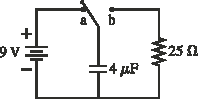
\includegraphics[width = 2in]{figures/rk2836.pdf}
\end{wrapfigure}

\item[\textbf{(28.36)}] Rofinn á myndinni hér til hægri hefur verið í stillingu $a$ í langan tíma. Við tímann $t = \SI{0}{s}$ er rofinn færður yfir í stillingu $b$. Hver verður hleðslan á þéttinum, $Q(t)$, og straumurinn í gegnum viðnámið, $I(t)$ \begin{enumerate*}[label = \textbf{(\alph*)}]
    \item einmitt þegar að rofanum er lokað?
    \item eftir $\SI{50}{\mu s}$
    \item eftir $\SI{200}{\mu s}$.
\end{enumerate*}

\end{minipage}

\vspace{1cm}

\begin{minipage}{\linewidth}
\begin{wraptable}{r}{1.5cm}
\vspace{-0.5cm}
\begin{tabular}{|c|c|}
        \hline
          $t \, \, [\si{s}]$   &  $I \, \, [\si{\mu A}]$ \\ \hline \hline
            \SI{0.5}{} & \SI{890}{} \\ \hline
            \SI{1.0}{} & \SI{640}{} \\ \hline
            \SI{1.5}{} & \SI{440}{} \\ \hline
            \SI{2.0}{} & \SI{270}{} \\ \hline
            \SI{2.5}{} & \SI{200}{} \\ \hline
        \end{tabular}
\end{wraptable}

\item[\textbf{(28.68)}] Þið eruð með fullhlaðinn \SI{20}{\mu F} þétti sem að þú tengir við tímann $t = \SI{0}{s}$ inn í rafrás með óþekkt viðnám. Í töflunni hér til hægri sjást straumgildin, $I$, sem að straummælirinn sýndi við tímann $t$. Gerið viðeigandi graf af gögnunum og ákvarðið viðnámið í rásinni og upphaflega spennufallið yfir þéttinn við tímann $t = \SI{0}{s}$.

\end{minipage}

\vspace{1cm}

\begin{minipage}{\linewidth}
\begin{wrapfigure}{r}{1.5in}
\vspace{-0.5cm}
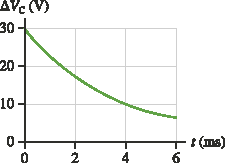
\includegraphics[width = 2in]{figures/rk2870.pdf}
\end{wrapfigure}

\item[\textbf{(28.70)}] Þéttir með rýmd \SI{50}{\mu F} hafði upphaflega verið hlaðinn þannig að spennumunurinn á milli platnanna var \SI{30}{V}. Grafið hér til hægri sýnir spennufallið, $\Delta V_C$, yfir þéttinn sem fall af tíma, $t$, þegar að þéttirinn er afhlaðinn í gegnum viðnám. Ákvarðið viðnámið, $R$.
\end{minipage}

\vspace{3cm}

\begin{minipage}{\linewidth}
\begin{wrapfigure}{r}{1.5in}
\vspace{-0.5cm}
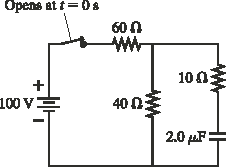
\includegraphics[width = 2in]{figures/rk2880.pdf}
\end{wrapfigure}

\item[\textbf{(28.80)}] Rofinn á myndinni hér til hægri hefur lokaður í langan tíma. Við tímann $t = \SI{0}{s}$ er rofinn opnaður.  \begin{enumerate*}[label = \textbf{(\alph*)}]
    \item Hver er hleðslan á þéttinum áður en rofinn er opnaður?
    \item Hversu langur tími líður þar til að hleðslan á þéttinum hefur minnkað niður í \SI{10}{\percent} af upphaflegu gildi sínu?
\end{enumerate*}

\end{minipage}

\end{enumerate}

\vspace{2cm}

\begin{tcolorbox}
\begin{enumerate*}[label = ]
  \item \textbf{(28.36)} $I(\SI{50}{\mu s}) = \SI{220}{mA}$, $I(\SI{200}{\mu s}) = \SI{49}{mA}$.
  \item \textbf{(28.68)} $R \approx \SI{64}{k\ohm}$, $I_0 \approx \SI{1180}{\mu A}$, $\Delta V_C(0) \approx \SI{75.5}{V}$.
  \item \textbf{(28.70)} $R = \SI{73}{\ohm}$.
  \item \textbf{(28.80)} $Q_0 = \SI{80}{\mu C}$, $t = \SI{230}{\mu s}$.
\end{enumerate*}
\end{tcolorbox}

\newpage

\subsection*{Dæmatími 28: LR-rásir}

\begin{tcolorbox}
$LR$-rás er rás sem að inniheldur einungis viðnám $R$ og spólu með spanstuðul $L$. Lykkjulögmálið gefur:
\begin{align*}
    - IR - L\frac{dI}{dt} = 0 \implies \frac{dI}{dt} + \frac{R}{L} I = 0 \implies I(t) = I_0e^{-Rt/L}
\end{align*}
Stærðin $\tau = \frac{L}{R}$ kallast stundum \emph{tímafasti} rásarinnar (sbr.~tímafasti RC-rásarinnar).
\end{tcolorbox}

\begin{enumerate}[label = \textbf{(\alph*)}]

\begin{minipage}{\linewidth}
\begin{wrapfigure}{r}{1.5in}
\vspace{-0.5cm}
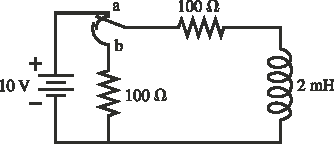
\includegraphics[width = 2in]{figures/rks3016.pdf}
\end{wrapfigure}

\item[\textbf{(30.16)}] Rofinn á myndinni hér til hægri hefur verið í stillingu $a$ í langan tíma. Við tímann $t = \SI{0}{s}$ er rofinn færður yfir í stillingu $b$. \begin{enumerate*}[label = \textbf{(\alph*)}]
    \item Hver er straumurinn í rásinni einmitt við tímann $t = \SI{0}{s}$?
    \item Hver verður straumurinn í rásinni við tímann $t = \SI{5.0}{\mu s}$?
    \item Við hvaða tíma mun straumurinn í rásinni hafa minnkað niður í \SI{1}{\percent} af upphaflegu gildi sínu?
\end{enumerate*}

\end{minipage}

\item[\textbf{(30.34)}] Lítum á rafrásina hér fyrir neðan til vinstri. Hvað gildi á $R$ gefur $\SI{25}{\mu s}$ tímafasta fyrir rafrásina?

\begin{figure}[H]
    \centering
    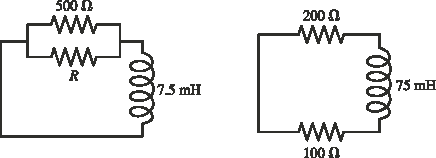
\includegraphics[scale = 1.25]{figures/rk3034.pdf}
\end{figure}

\item[\textbf{(30.35)}] Lítum á rafrásina hér fyrir ofan til hægri. Við tímann $t = \SI{0}{s}$ er straumurinn í rásinni $I_0$. Við hvaða tíma veðrur straumurinn í rásinni $\frac{1}{2}I_0$?

\begin{comment}
\item[\textbf{(30.76)}] Lítum á rafrásina hér fyrir neðan til vinstri. Rofinn hefur verið opinn í langan tíma. Við tímann $t = \SI{0}{s}$ er rofanum lokað. Hver verður straumurinn sem að fer í gegnum \SI{20}{\ohm} viðnámið \begin{enumerate*}[label = \textbf{(\alph*)}]
    \item um leið og rofanum er lokað?
    \item eftir að rofinn hefur verið lokaður í langan tíma?
    \item um leið og rofinn er opnaður aftur?
\end{enumerate*}

\begin{figure}[H]
    \centering
    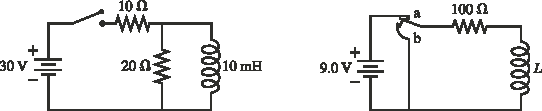
\includegraphics[scale = 1.25]{figures/rk3078.pdf}
\end{figure}

\begin{minipage}{\linewidth}
\begin{wraptable}{r}{1.5cm}
\vspace{-1.5cm}
\begin{tabular}{|c|c|}
        \hline
          $t \, \, [\si{\mu s}]$   &  $\Delta V_R \, \, [\si{V}]$ \\ \hline \hline
            \SI{0}{} & \SI{9.0}{} \\ \hline
            \SI{10}{} & \SI{6.7}{} \\ \hline
            \SI{20}{} & \SI{4.6}{} \\ \hline
            \SI{30}{} & \SI{3.2}{} \\ \hline
            \SI{40}{} & \SI{2.5}{} \\ \hline
        \end{tabular}
\end{wraptable}
\item[\textbf{(30.78)}] Lítum á rafrásina hér fyrir ofan til hægri. Við tímann $t = \SI{0}{s}$ er rofinn færður úr stöðu $a$ í stöðu $b$. Með því að nota spennumæli þá mælum við spennufallið í gegnum viðnámið, $\Delta V_R$, sem fall af tíma, $t$. Niðurstöður mælinganna er að finna hér í töflunni til hægri. Ákvarðið spanstuðul spólunnar með því að gera viðeigandi graf af gögnunum.

\end{minipage}

\end{comment}

\vspace{0.3cm}

\begin{minipage}{\linewidth}
\begin{wrapfigure}{r}{1.5in}
\vspace{-0.5cm}
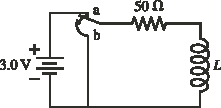
\includegraphics[width = 2in]{figures/rk3079.pdf}
\end{wrapfigure}

\item[\textbf{(30.79)}] Lítum á rafrásina hér til hægri. Við tímann $t = \SI{0}{s}$ er rofinn færður úr stöðu $a$ í stöðu $b$. Við tímann $t = \SI{5.0}{\mu s}$ hefur spólan tapað helmingnum af orkunni sem að hún geymdi við tímann $t = \SI{0}{s}$. Hvert er gildið á spanstuðli spólunnar?

\end{minipage}


\end{enumerate}

\vspace{0.75cm}

\begin{tcolorbox}
\begin{enumerate*}[label = ]
  \item \textbf{(30.16)} $I_0 = \SI{0.10}{A}$, $I(\SI{5.0}{\mu s}) = \SI{61}{mA}$, $t = \SI{46}{\mu s}$.
  \item \textbf{(30.34)} $\SI{750}{\ohm}$.
  \item \textbf{(30.35)} $\SI{173}{\mu s}$. \\
  \item \textbf{(30.79)} $L = \SI{720}{\mu H}$.
\end{enumerate*}
\end{tcolorbox}

\newpage

\subsection*{Dæmatími 29: LC-rásir}

\begin{tcolorbox}
$LC$-rás er rás sem að inniheldur einungis spólu með spanstuðul $L$ og þétti með rýmd $C$. Fáum þá:
\begin{align*}
    \frac{Q}{C} - L \frac{dI}{dt} = 0 \implies \frac{d^2Q}{dt^2} + \frac{1}{LC} Q = 0 \implies Q(t) = Q_{\text{max}}\cos(\omega t + \varphi), \hspace{0.3cm} \omega = \frac{1}{\sqrt{LC}}
\end{align*}
Sem er einfaldlega einföld sveifluhreyfing. Fasahornið ákvarðast af upphafsskilyrðunum og rafstraumurinn fæst með því að diffra hleðsluna. Stærðin $\omega = \frac{1}{\sqrt{LC}}$ kallast sveiflutíðni rásarinnar.
\end{tcolorbox}

\begin{enumerate}[label = \textbf{(\alph*)}]

\item[\textbf{(30.71)}] Þú hefur fengið $LC$-rás í jólagjöf frá ömmu þinni (þú baðst reyndar um $RC$-rás). Amma þín keypti spólu með spanstuðul $\SI{20}{mH}$ og plötuþétti með rýmd \SI{8.0}{pF}. Amma þín var búin að hlaða plötur plötuþéttisins þannig að spennumunurinn á milli platna plötuþéttisins er \SI{25}{V}. Þú tengir síðan rásina á aðfangadag við tímann $t = \text{18:00}$. \begin{enumerate*}[label = \textbf{(\alph*)}]
    \item Hversu langur tími mun líða þar til að þéttirinn er alveg afhlaðinn í fyrsta skipti?
    \item Hver verður straumurinn sem að fer í gegnum spóluna einmitt þá?
\end{enumerate*}

\item[\textbf{(30.72)}] Spennufallið yfir þétti með rýmd \SI{0.10}{\mu F} er \SI{5.0}{V}. Við tímann $t = \SI{0}{s}$ er þéttirinn tengdur við spólu með spanstuðul $\SI{1.0}{mH}$. Hver verður mesti straumurinn sem að fer í gegnum spóluna í sveifluhreyfingunni?

\item[\textbf{(30.73)}] Sem hluti af munnlegu prófi í eðlisfræði þá biður erfiði eðlisfræðikennarinn þinn þig um að búa til $LC$-rás sem að sveiflast með tíðni $\SI{10}{kHz}$. Sem varúðarráðstöfun þá biður hann þig þar að auki um að sjá til þess að mesti straumurinn í rásinni sé $\SI{0.10}{A}$ og að mesta orkan sem að þéttirinn geymir sé $\SI{1.0e-5}{J}$. Hver á rýmd þéttisins að vera og hver á spanstuðull spólunnar að vera?

\begin{minipage}{\linewidth}
\begin{wrapfigure}{r}{1.5in}
\vspace{-0.5cm}
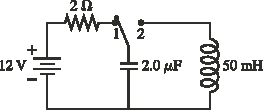
\includegraphics[width = 2in]{figures/rk3033c.pdf}
\end{wrapfigure}

\item[\textbf{(30.33)}] Rofinn á myndinni hér til hægri hefur verið í stillingu 1 í langan tíma. Hann er færður yfir í stillingu 2 við tímann $t = \SI{0}{s}$. \begin{enumerate*}[label = \textbf{(\alph*)}]
    \item Hver verður mesti straumurinn sem að fer í gegnum spóluna?
    \item Við hvaða tíma verður straumurinn mestur (í fyrsta skipti) í spólunni?
\end{enumerate*}

\vspace{1cm}

\end{minipage}


\begin{comment}
\begin{minipage}{\linewidth}
\begin{wrapfigure}{r}{1.5in}
\vspace{-0.5cm}
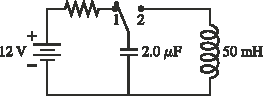
\includegraphics[width = 2in]{figures/rk3033.pdf}
\end{wrapfigure}

\item[\textbf{(30.75)}] Í rásinni hér til hægri sést fullhlaðinn \SI{300}{\mu F} þéttir og óhlaðinn \SI{1200}{\mu F} þéttir. Spennufallið yfir \SI{300}{\mu F} þéttinn er til að byrja með \SI{100}{V}. Til að byrja með eru báðir rofarnir opnir og enginn straumur hleypur í rásinni. Ef að þú mættir opna og loka rofunum að vild við hvaða tíma sem er, hver væri þá mesta hleðslan sem að þú gætir komið fyrir á \SI{1200}{\mu F} þéttinum? Hver væri minnsti tíminn sem að það tæki það þig að fullhlaða \SI{1200}{\mu F} þéttinn?

\end{minipage}
\end{comment}

\end{enumerate}

\begin{tcolorbox}
\begin{enumerate*}[label = ]
  \item \textbf{(30.71)} $t = \SI{628}{ns}$, $\SI{500}{\mu A}$.
  \item \textbf{(30.72)} $I_{\text{max}} = \SI{50}{mA}$.
  \item \textbf{(30.73)} $C = \SI{130}{nF}$, $L = \SI{2.0}{mH}$. \\
  \item \textbf{(30.33)} $I_{\text{max}} = \SI{76}{mA}$, $t = \SI{500}{\mu s}$.
\end{enumerate*}
\end{tcolorbox}

\newpage

\subsection*{Dæmatími 30: RCL-rásir með AC-spennugjafa}

\begin{tcolorbox}
$RCL$-sveiflurásir eru rásir sem innihalda sveifluspennugjafa $\mathcal{E}(t) = \mathcal{E}_0\cos(\omega t)$ sem er raðtengdur við viðnám, $R$, spólu með spanstuðul, $L$ og þétti með rýmd, $C$. Lögmál Kirchoffs gefa þá að:
\begin{align*}
    \mathcal{E}(t) - \Delta V_R - \Delta V_L - \Delta V_C = 0
\end{align*}
Með því að leysa þessa diffurjöfnu fæst að straumurinn í rásinni er gefinn með:
\begin{align*}
    I(t) = I_0 \cos(\omega t - \varphi), \hspace{0.5cm} \text{þar sem} \hspace{0.5cm} \varphi = \arctan\left(\frac{X_L-X_C}{R}\right).
\end{align*}
Þar að auki sem:
\begin{align*}
    I_0 = \frac{\mathcal{E}_0}{Z}, \hspace{1cm} Z = \sqrt{R^2 + (X_L - X_C)^2}, \hspace{1cm} X_L = \omega L, \hspace{1cm} X_C = \frac{1}{\omega C}.
\end{align*}
Í þessum fræðum er líka oft fjallað um svokölluð \emph{rms}-gildi. Þá skilgreinum við:
\begin{align*}
    \mathcal{E}_{\text{rms}} = \frac{\mathcal{E}_0}{\sqrt{2}}, \hspace{0.8cm} I_{\text{rms}} = \frac{I_0}{\sqrt{2}}.
\end{align*}
Aflið sem að sveifluspennugjafinn gefur tapast síðan í viðnáminu og meðalaflið sem að tapast er:
\begin{align*}
    P = \mathcal{E}_{\text{rms}} I_{\text{rms}} \cos\varphi.
\end{align*}
\end{tcolorbox}

\begin{enumerate}[label = \textbf{(\alph*)}]

\begin{minipage}{\linewidth}
\begin{wrapfigure}{r}{1.5in}
\vspace{-0.5cm}
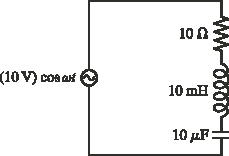
\includegraphics[width = 2in]{figures/rk3232.pdf}
\end{wrapfigure}


\item[\textbf{(32.30)}] Raðtengd $RLC$-rás samanstendur af \SI{50}{\ohm} viðnámi, \SI{3.3}{mH} spólu og \SI{480}{nF} þétti. Hún er tengd við sveifluspennu með útslag $\SI{5.0}{V}$. Ákvarðið samviðnám ($Z$) rásarinnar, stærsta gildið á straumnum í rásinni, fasahornið og meðalaflið við eftirfarandi gildi á tíðninni: \begin{enumerate*}[label = \textbf{(\alph*)}]
    \item \SI{3000}{Hz} \item \SI{4000}{Hz}
\end{enumerate*}

\item[\textbf{(32.32)}] Lítum á rásina hér til hægri. \begin{enumerate*}[label = \textbf{(\alph*)}]
    \item Hver er hermitíðni rásarinnar? (Ath. við segjum að rásin sé við \emph{hermitíðni} ef að \emph{samviðnám rásarinnar}, $Z = R$ en þá er $X_L = X_C$).
    \item Hvert er fasahornið við hermitíðnina?
    \item Hvert er meðalaflið sem að tapast í rásinni við hermitíðnina?
\end{enumerate*}

\end{minipage}

\vspace{0.25cm}

\item[\textbf{(32.52)}] Raðtengd $RLC$-rás samanstendur af \SI{550}{\ohm} viðnámi, \SI{0.10}{H} spólu og \SI{100}{\mu F} þétti. Hún tekur \SI{2.5}{A} rms-straum þegar að hún er tengd við \SI{60}{Hz} sveifluspennugjafa. Hver eru gildin á: \begin{enumerate*}[label = \textbf{(\alph*)}]
    \item rms-spennunni, $\mathcal{E}_{\text{rms}}$
    \item fasahorninu, $\varphi$?
    \item Meðalaflinu sem að tapast í rásinni?
\end{enumerate*}

\item[\textbf{(32.53)}] Raðtengd $RLC$-rás samanstendur af \SI{550}{\ohm} viðnámi, $\SI{2.1}{mH}$ spólu og \SI{550}{nF} þétti. Hún er tengd við \SI{50}{V} rms-spennugjafa sem er hægt að stilla sveiflutíðnina á. Í \SI{2.5}{mm} fjarlægð frá einum af vírunum í rásinni má greina segulsvið sem að sveiflast vegna riðstraumsins í rásinni. Hvert er stærsta gildið á segulsviðinu sem að er hægt að búa til og við hvaða sveiflutíðni er það?

\end{enumerate}

\begin{tcolorbox}
\begin{enumerate*}[label = ]
  \item \textbf{(32.30)} $Z_a = \SI{179.8}{\ohm}, I_a = \SI{27.8}{mA}, \varphi_a = \SI{1.29}{rad}, P_a = \SI{19.3}{mW}$. \\  $Z_b =\SI{173.2}{\ohm}, I_b = \SI{28.9}{mA}, \varphi_b = \SI{1.28}{rad}, P_b = \SI{20.7}{mW}$.
  \item \textbf{(32.32)} $f = \SI{503}{Hz}$, $\varphi = \SI{0}{rad}$, $P = \SI{5.0}{W}$.
  \item \textbf{(32.52)} $\mathcal{E}_{\text{rms}} = \SI{128}{V}$, $\varphi = \SI{0.22}{rad}$, $P = \SI{312}{W}$.
  \item \textbf{(32.53)} $B_{\text{max}} = \SI{7.3}{\mu T}$, $f = \SI{4680}{Hz}$.
\end{enumerate*}
\end{tcolorbox}

\newpage

%%%%%%%%%%%%%%%%%%%%%%%%%%%%%%%%
%      END OF CHAPTER TEXT 
%%%%%%%%%%%%%%%%%%%%%%%%%%%%%%%%
\ifdefined \wholebook \else
 \printindex
\end{document}
\fi